% !TeX root = ../thuthesis-example.tex

\chapter{引言}


\section{研究背景}

网络自诞生以来,随着数十年的发展,已经成为了最重要的信息化基础设施之一。如图~\ref{fig:example}所示,第46次《中国互联网络发展状况统计报告》\cite{cac.gov} 指出,截至2020年6月,我国网民规模达到9.40亿,互联网普及率达67.0\%,
互联网应用涵盖即时通讯、搜索引擎、网络新闻、 在线教育、购物出行等方面,可以说互联网已经和每个人的生活息息相关密不可分。

\begin{figure}
    \centering
    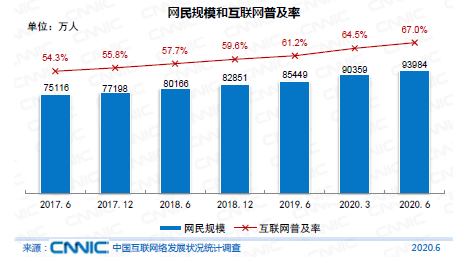
\includegraphics[width=0.6\linewidth]{网民规模.PNG}
    \caption{网民规模和互联网普及率}
    \label{fig:example}
  \end{figure}

随着网络重要性的提升、用户规模的膨胀,管理网络的难度也越来越大。网络是一个复杂的系统,它的部署、运行和维护都需要专业的运维人员。
早期的运维工作大部分是由运维人员手工完成,然后人们逐渐发现一些重复性的工作可以用自动化脚本来实现,于是诞生了自动化运维。自动化运维可以认为是基于专家经验、人为制定规则的系统。
但是随着互联网规模急剧膨胀,以及服务类型的多样化,简单的、基于人为制定规则的方法并不能解决大规模运维的问题,因此产生了智能运维。与自动化运维依赖专家知识、人工生成规则不同,
智能运维强调使用机器学习算法从海量运维数据中不断学习、不断提炼规则。

异常检测是智能运维的关键环节,具有至关重要的意义。从网络故障管理的角度来说,做好异常检测可以提前预测故障的发生;从性能管理的角度来说,可以发现性能不佳的区域,避免因误配置、架构不合理导致性能下降;
从安全管理的角度来说,在网络攻击的前期阶段,及时发现并预警后续攻击,进而做出防御措施。因此,在复杂的网络环境中甄别出有效和异常流量尤为重要,在重大事故发生前,
根据各项流量特征的变化,提前预测出即将发生的事故,提高应急响应速度,防患于未然。


% 接下来我们将以校园网为例,进行异常检测算法和系统的研究。清华大学校园网是全球规模最大,架构最复杂,流量场景最多变的校园网之一,具有以下几个特点:
% 1.	用户规模大,流量峰值高。每天有10万台设备活跃在线,同时在线设备最多为7万台,峰值流量约为30Gbps/s.
% 2.	用户应用类型多,远比一般的企业网复杂,在网络环境中几百种应用同时使用,这给数据分析带来了很多困难。
% 3.	异常流量是常态。扫描流量、攻击流量占比多。
% 这些特点给异常检测的研究和实现带来了诸多挑战。

\section{研究内容}

\section{主要贡献}

\section{论文组织结构}